\section{Einführung}
\label{sec:Einführung}
Diese Arbeit befasst sich grundlegend mit dem Fussgänger-Routing und dem Auffinden der nächsten ÖV-Haltestelle, welche einem an ein weiter gelegenes Ziel führen kann. Ziel ist es von einem gegebenen Punkt die nächste ÖV-Haltestelle, welche zu Fuss erreichbar ist, zu finden. Im folgenden ist die Problemstellung erläutert und es wird eine Abgrenzung gemacht, was Teil dieser Arbeit ist.

\subsection{Problemstellung und Vision}
\label{sub:Problemstellung und Vision}
%TODO Verweis auf GraphHopper?
Die heutig gängigen Routing-Engines können effizient über Kanten und Knoten routen und navigieren, um so den schnellstmöglichen Weg finden zu können. Diese wurden stetig für Autofahrer optimiert, da sich diese unter anderem an vorgegebene Regeln halten. Beim nicht-motorisierten Individualverkehr (Fussgänger, Rollstuhlfahrer, Radfahrer, etc.)  ist das nicht immer der Fall. In den folgenden Unterkapiteln werden einige Probleme erläutert, welche immer noch Praxis für den nicht-motorisierten Individualverkehr sind.

\subsubsection{Routing über offene Flächen}
\label{subsub:Routing über offene Flächen}
Wie man an in der Abbildung \ref{fig:helvetiaplatz_graphhopper} gut sieht, routet die Routing-Engine GraphHopper den Kanten nach um den Platz herum. Dies ist ein natürliches Verhalten für den motorisierten Individualverkehr. Ein Fussgänger hingegen nimmt den direkten Weg über den Platz. Oft handelt es sich nicht nur um einen leeren Platz, sondern es sind darauf Hindernisse, wie Brunnen, Kunstwerke, WCs, etc. stationiert, um welche auf eine natürliche Weise geroutet werden muss. Eine Route, welche direkt auf das Hindernis routet, und dann um das Hindernis herumläuft ist zwar ein Fortschritt zur aktuellen Lösung, entspricht aber keinem normalen Fussgänger-Verhalten. 

\begin{figure}[ht]
	\centering
	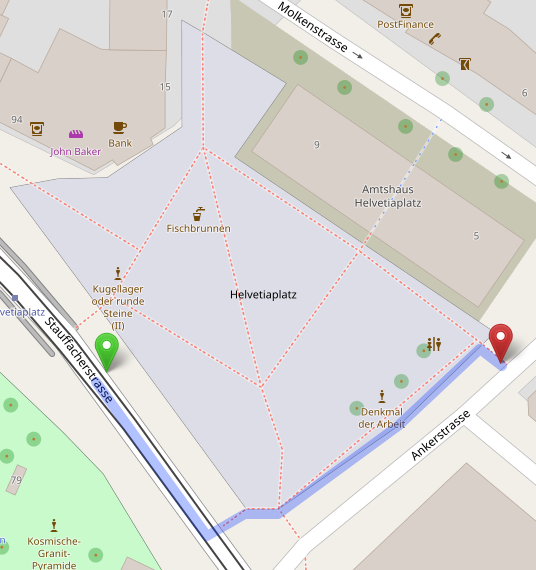
\includegraphics[width=0.5\linewidth]{technicalreport/img/helvetiaplatz_graphhopper}
	\caption[Fussgänger-Routing]{Fussgänger-Routing mit GraphHopper über den Helvetiaplatz, Zürich, Schweiz; Screenshot von openstreetmap.org aufgenommen am 08.10.2017}
	\label{fig:helvetiaplatz_graphhopper}
\end{figure}

\subsubsection{eingezeichnete Fussgängerrouten über offene Flächen}
\label{subsub:eingezeichnete Fussgängerrouten über offene Flächen}
Wenn man die gleiche Abbildung \ref{fig:helvetiaplatz_graphhopper} nochmals betrachtet, sieht man, dass Mapper bereits einige Fussgängerwege auf dem Platz eingezeichnet haben, um dem Routing-Problem über offene Fläche entgegen zu steuern. Dies kann in einigen Situationen, wie dem Helvetiaplatz kontraproduktiv, aber in anderen wieder von Vorteil sein. Betrachtet man beispielsweise den Central Park in New York in Abbildung \ref{fig:central_park} macht es Sinn, dass das Routing den vorgegeben Wegen folgt. Eine Wiese gilt als offene Fläche, eignet sich aber nicht immer als vorteilhafter Bewegungsuntergrund. Man muss abklären, in welchen Situation man sich auf gemappte Wege über offene Wege verlassen kann und wann sie zu ignorieren sind.

\begin{figure}[ht]
\centering
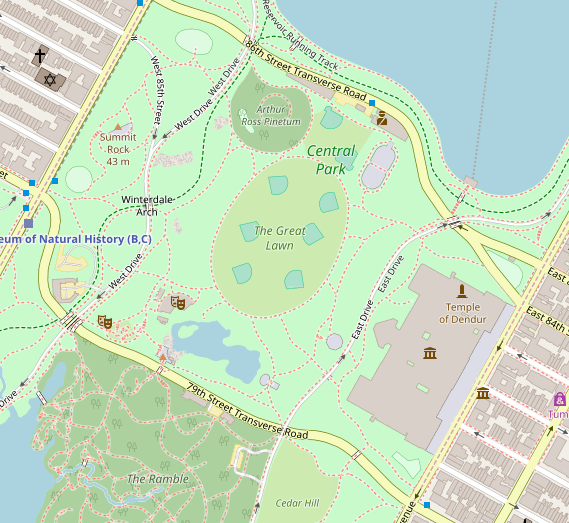
\includegraphics[width=0.5\linewidth]{technicalreport/img/central_park}
\caption[eingezeichnete Fussgänger-Routen]{Eingezeichnete Fussgänger-Routen auf dem Central Park, New York City, USA; Screenshot von openstreetmap.org aufgenommen am 08.10.2017}
\label{fig:central_park}
\end{figure}


\subsubsection{topologisch nicht verbundene Wege}
\label{subsub:topologisch nicht verbundene Wege}

\begin{figure}[ht]
\centering
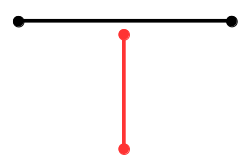
\includegraphics[width=0.5\linewidth]{technicalreport/img/topologisch_nicht_verbundener_graph}
\caption[topologisch nicht verbundener Graph]{topologisch nicht verbundener Graph}
\label{fig:topologisch_nicht_verbundener_graph}
\end{figure}

In Abbildung \ref{fig:topologisch_nicht_verbundener_graph} ist ein topologischer nicht verbundener Graph zu sehen. In OSM kann es vorkommen, dass solche Wege auf eine offene Fläche treffen, mit dieser aber nicht konkret verbunden sind. Eine Routing-Engine muss in der Lage sein, dies zu erkennen und aufzuräumen, so dass vom auftreffenden Weg über die offene Fläche geroutet werden kann.

\subsubsection{Routing über über weitere Arten von offenen Flächen (Berge, Strände)}
\label{subsub:Routing über über weitere Arten von offenen Flächen (Berge, Strände)}
Berge und Strände sind bekanntermassen schwieriger zu überqueren als normale Plätze. Sei dies aufgrund der zurückzulegenden Höhendifferenz oder die Unterlage, welche das Fortbewegen mühsamer macht. Zusätzlich zum Problem \ref{subsub:Routing über offene Flächen} kommt hier dazu, dass Umlaufen dieser offene Fläche (Berge, Strände) effizienter sein kann, als das Überqueren.  
	
\subsection{Ziele und Unterziele}
\label{sub:Ziele und Unterziele}

\subsubsection{Routing über offene Flächen}
\label{subsub:Ziel Routing über offene Flächen}
Das Problem \ref{subsub:Routing über offene Flächen} wurde bereits in einigen Arbeiten \cite{graser_visibility_graph}, \cite{dzafic_spider_web_graph}  aufgegriffen, auf welche Bezug genommen wird. Diese beiden Ansätze (Visibility-Graph und SpiderWeb-Graph) werden analysiert, Tests in QGIS implementiert und getestet. Ziel ist es, die optimale Variante, um über offene Flächen den schnellstmöglichen Weg zu finden, zu eruieren. 

\subsubsection{Routing-Engine evaluieren}
\label{subsub:Ziel Routing-Enginge evaluieren}
Die zahlreichen Routing-Engines sollen analysiert und festgehalten werden, welche sich für den Hauptzweck dieser Arbeit am besten eignet. Zusätzlich wird geprüft, wie die Datenvorverarbeitung (Einzeichnen der Routen für Routing über offene Flächen) in die bestehenden Routing-Engines eingehängt werden kann. 

\subsubsection{eingezeichnete Fussgängerrouten über offene Flächen}
\label{subsub:Ziel eingezeichnete Fussgängerrouten über offene Flächen}
Es soll eruiert werden, ob für den Platz die eingezeichneten Fussgängerrouten ignoriert werden können oder ob man an diese gebunden ist, wie man in Abbildung \ref{fig:central_park} sieht.

\subsubsection{topologisch nicht verbundene Wege}
\label{Ziel subsub:topologisch nicht verbundene Wege}
TODO: was wird in unserer Arbeit hier gemacht?

\subsubsection{Routing über über weitere Arten von offenen Flächen (Berge, Strände)}
\label{subsub:Ziel Routing über über weitere Arten von offenen Flächen (Berge, Strände)}
Im Kontext dieser Arbeit wird ein theoretischer Ansatz aufgezeigt, wie man mit einem kostenbasierten Graph den Eigenschaften diesen Unterflächen gerecht wird.

\subsection{nächste ÖV-Haltestelle finden}
\label{subsub:Ziel nächste ÖV-Haltestelle finden}
Der Fokus der Arbeit liegt auf dem Finden und Erreichen der nächsten ÖV-Haltestelle, welche einem ans gewünschte Ziel führt. So soll eruiert werden, wie von einem bestehenden Startpunkt die nächsten ÖV-Haltestellen identifiziert werden, um diese an search.ch für das weitere Routing zu übergeben.
	
\subsection{Rahmenbedingungen, Umfeld, Definitionen, Abgrenzungen}
\label{sub:Rahmenbedingungen, Umfeld, Definitionen, Abgrenzungen}
TODO

\subsection{Vorgehen und Aufbau der Arbeit}
\label{sub:Vorgehen und Aufbau der Arbeit}
TODO
